 % % % % % % % % % % % % % % % % % % % % % % % % % % % % % % % % % % % %
 % % % % % % % % % % % % % % % % % % % % % % % % % % % % % % % % % % % %
 % % % % % % % % % % % % % % % % % % % % % % % % % % % % % % % % % % % %

\documentclass[paper=a4, fontsize=12pt]{scrartcl} 
\usepackage[T1]{fontenc} 
\usepackage{geometry}

\usepackage[utf8]{inputenc}
\usepackage[english]{babel}
 
\usepackage[nottoc]{tocbibind}
\usepackage{fourier} 
\usepackage{float}
\usepackage{graphicx}
\usepackage[english]{babel} 
\usepackage{amsmath,amsfonts,amsthm} 
\usepackage{listings}
\usepackage{sectsty} 
\allsectionsfont{\centering \normalfont\scshape} 
\usepackage{fancyhdr} % Custom headers and footers
\usepackage{float}

 % % % % % % % % % % % % % % % % % % % % % % % % % % % % % % % % % % % %

\pagestyle{fancyplain} 
\geometry{legalpaper, margin=1.3in}

\fancyhead{} 
\fancyfoot[L]{} 
\fancyfoot[C]{} 
\fancyfoot[R]{\thepage} 
\renewcommand{\headrulewidth}{0pt} 
\renewcommand{\footrulewidth}{0pt} 
\setlength{\headheight}{13.6pt} 
\numberwithin{equation}{section} 
\numberwithin{figure}{section} 
\numberwithin{table}{section}
\setlength\parindent{0pt} 

 % % % % % % % % % % % % % % % % % % % % % % % % % % % % % % % % % % % %

\newcommand{\horrule}[1]{\rule{\linewidth}{#1}}  
 
 % % % % % % % % % % % % % % % % % % % % % % % % % % % % % % % % % % % %

\title{	
\normalfont \normalsize 
\textsc{Barcelona Graduate School of Economics - Data Science} \\ [25pt]
\horrule{2pt} \\[0.5cm] 
\huge Deep Feature Learning for (Random) Forest Cover Type Prediction  \\ 
\horrule{2pt} \\[0.5cm] 
}


\author{J\'essica Leal, Tim Kreienkamp and Philipp Schmidt} 
\date{}



 % % % % % % % % % % % % % % % % % % % % % % % % % % % % % % % % % % % %


\begin{document}



 % % % % % % % % % % % % % % % % % % % % % % % % % % % % % % % % % % % %


\maketitle
\textbf{Abstract:} \\
From a seven-class training data with 50,000 observations we try to find the best predictive model using different Machine Learning algorithm such as K-nearest neighbors, GBM, Support Vector Machine, Random Forest and Random Forest with deep learning. Our aim is to best predict this seven-class data set with 100,000 observations. For each model, we perform a 10-fold cross validation in order to assess the performance of our classifier in the training data set. After estimating the best hyperparameters for each model - with cross-validation - and comparing the train performance, we consider the Random Forest with deep feature learning is the best type of algorithm which can predict better our data. 


 % % % % % % % % % % % % % % % % % % % % % % % % % % % % % % % % % % % %



\section{Introduction}
\subsection{Dataset Characteristics}
In this project, we work with a training data set of 50,000 observations - with labels - and a testing set - without labels - of 100,000 observations. Our aim is to predict a seven-class variable in which each label is a different type of forest cover using cartographic variables. We have 10 numeric variables presented in a raw manner that needed to be scaled, and 44 binary variables for qualitative aspects of the forest such as the wilderness of that forest and the type of soil. 

 % % % % % % % % % % % % % % % % % % % % % % % % % % % % % % % % % % % %
\subsection{Baseline}
Before considering a unique and a priori thought best classifier, we attempted to model our data with different other classifier such as the K-NN and the SVM in order to mark us a benchmark for future steps in classification.


 % % % % % % % % % % % % % % % % % % % % % % % % % % % % % % % % % % % %
\newpage
\section{Exploratory Analysis}
The exploratory analysis is conducted to develop a thorough understanding of the dataset, to find relationships between the features and suggest new variables that might help to predict forest cover type. Within this report we focus on relationships among features and the creation of new variables. A more elaborate feature exploration is presented in an additional markdown file.

\subsection{Relation between features}
We use scatterplots to observe the relationships between the quantitative features.\\

\begin{figure}[H]
    \centering
    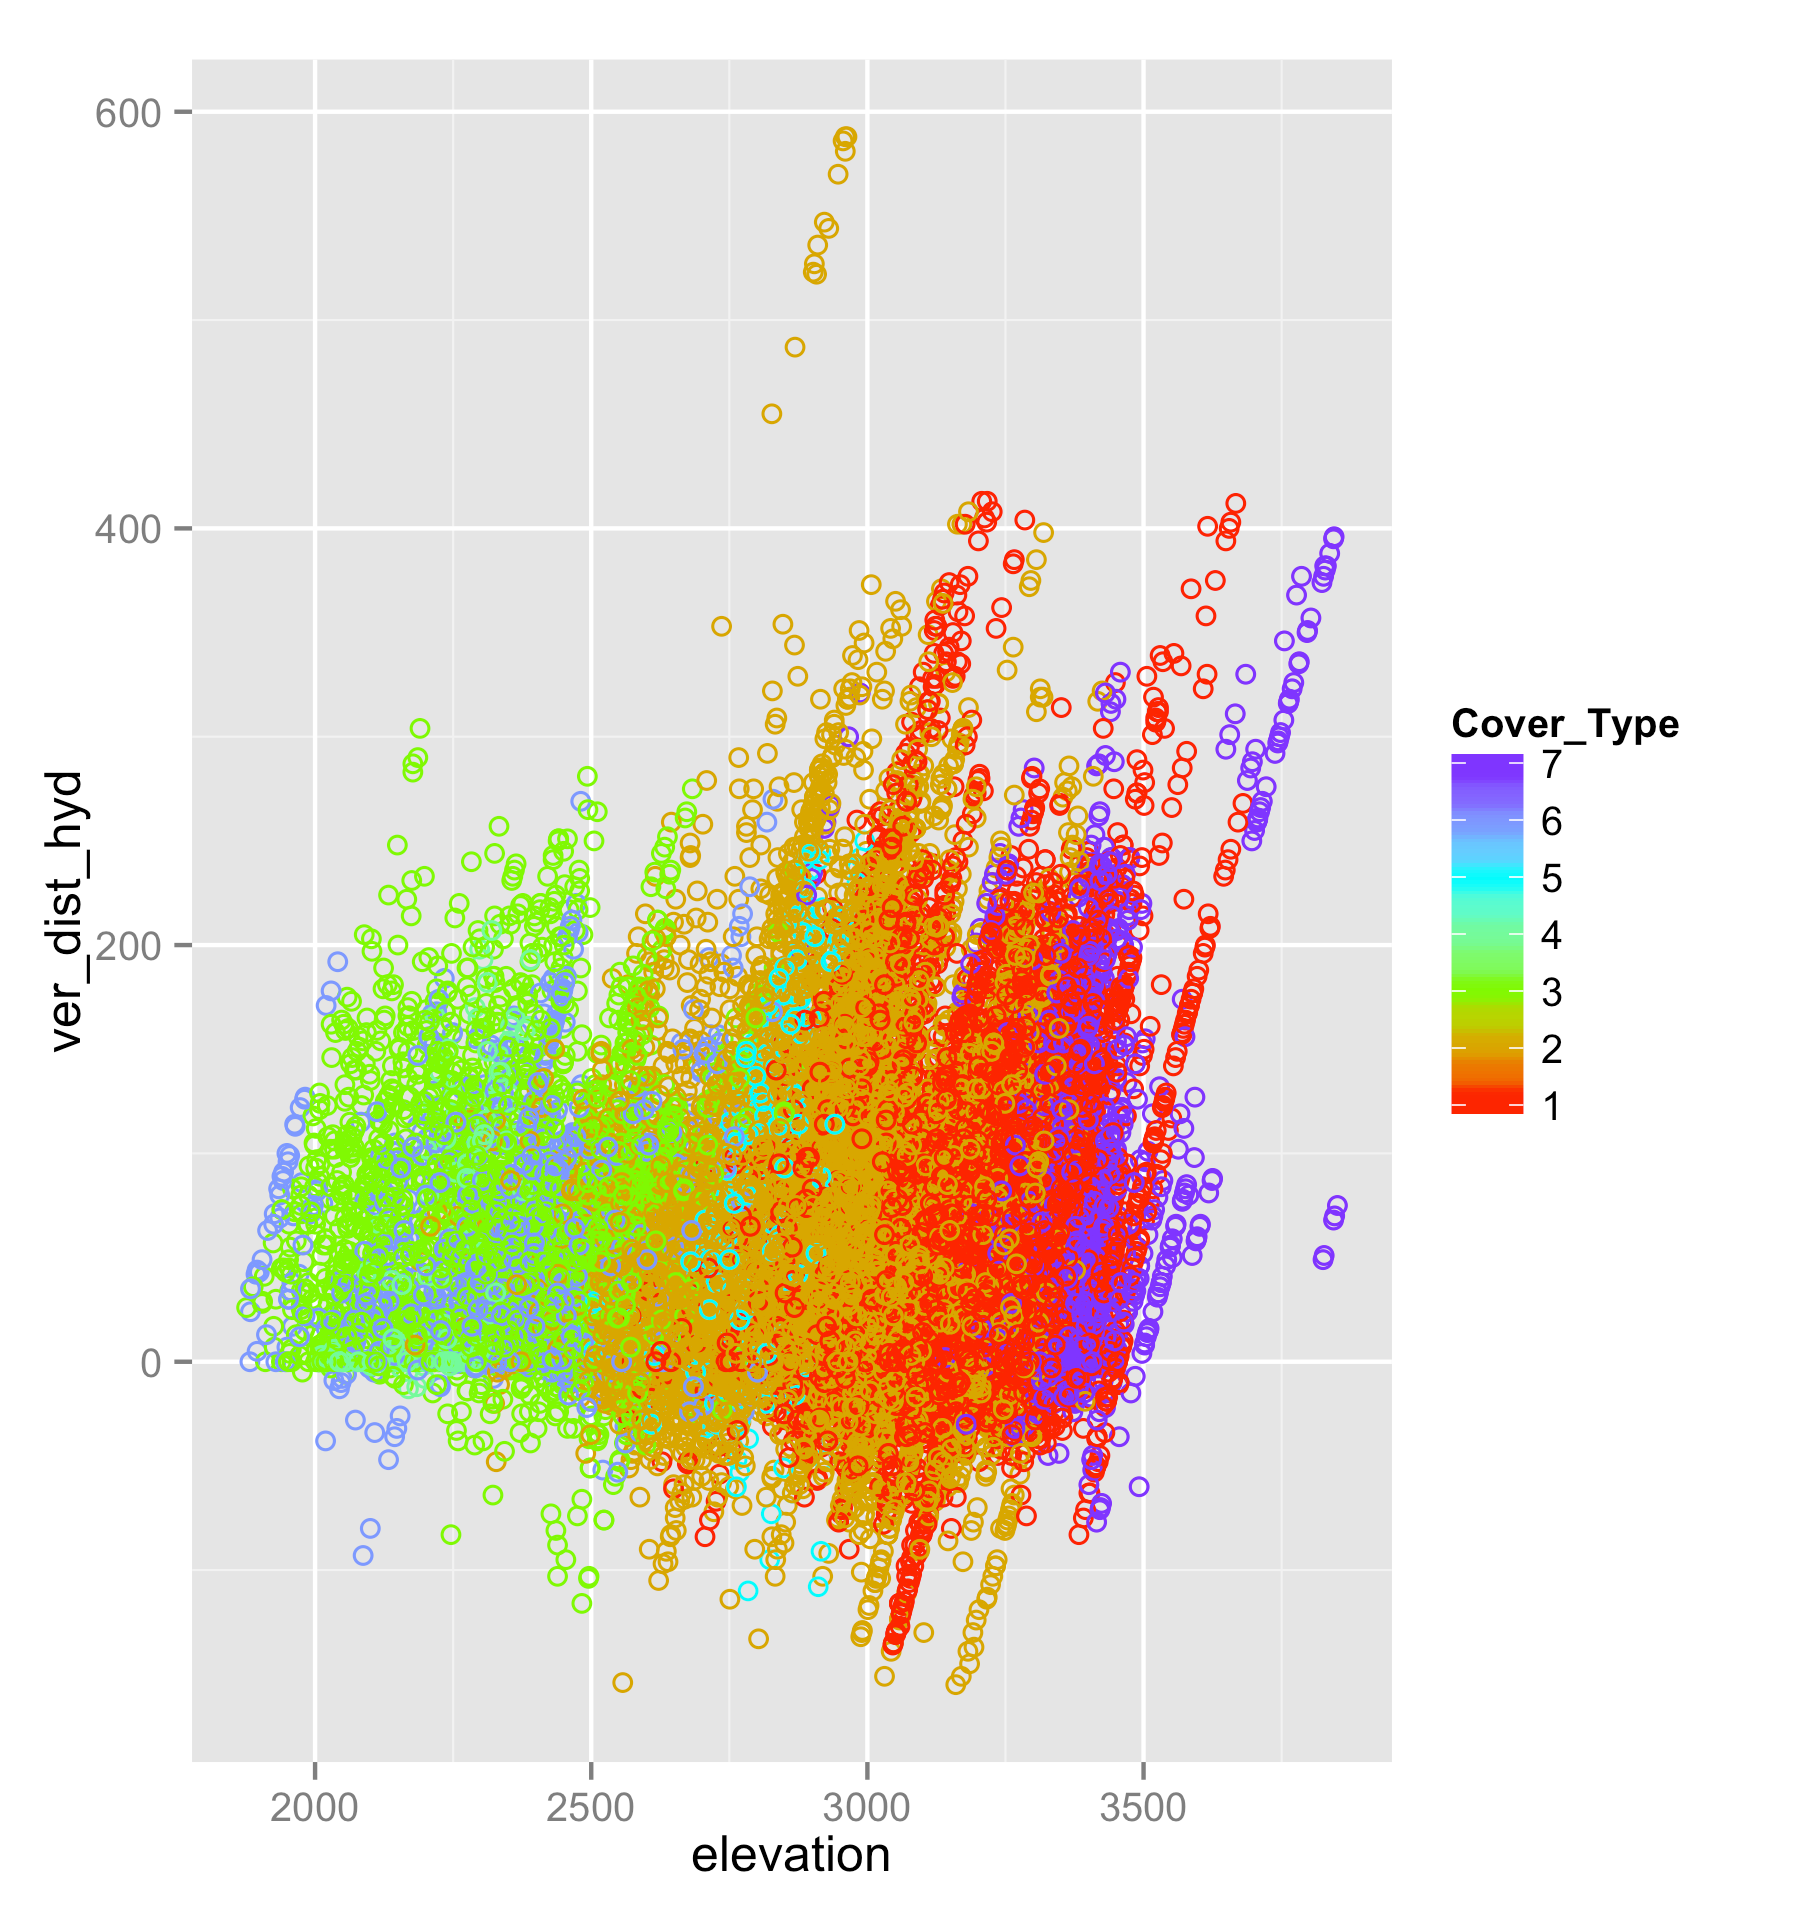
\includegraphics[width=0.8\textwidth]{elevation_ver.png}
    \caption{ \textbf{Plotting elevation vs. \lstinline{vert_dist_hyd}}}
    \label{fig:errors}
\end{figure}

There appears to be a strong relationship between the vertical distance and elevation within the groups. We thus create a new variable to account for this relationship which will later be tested for its predictive power. \\

Variable creation 1 (EVTH)
\begin{lstlisting}
data$EVTH <-  data$elevation - data$ver_dist_hyd
\end{lstlisting}

\begin{figure}[H]
    \centering
    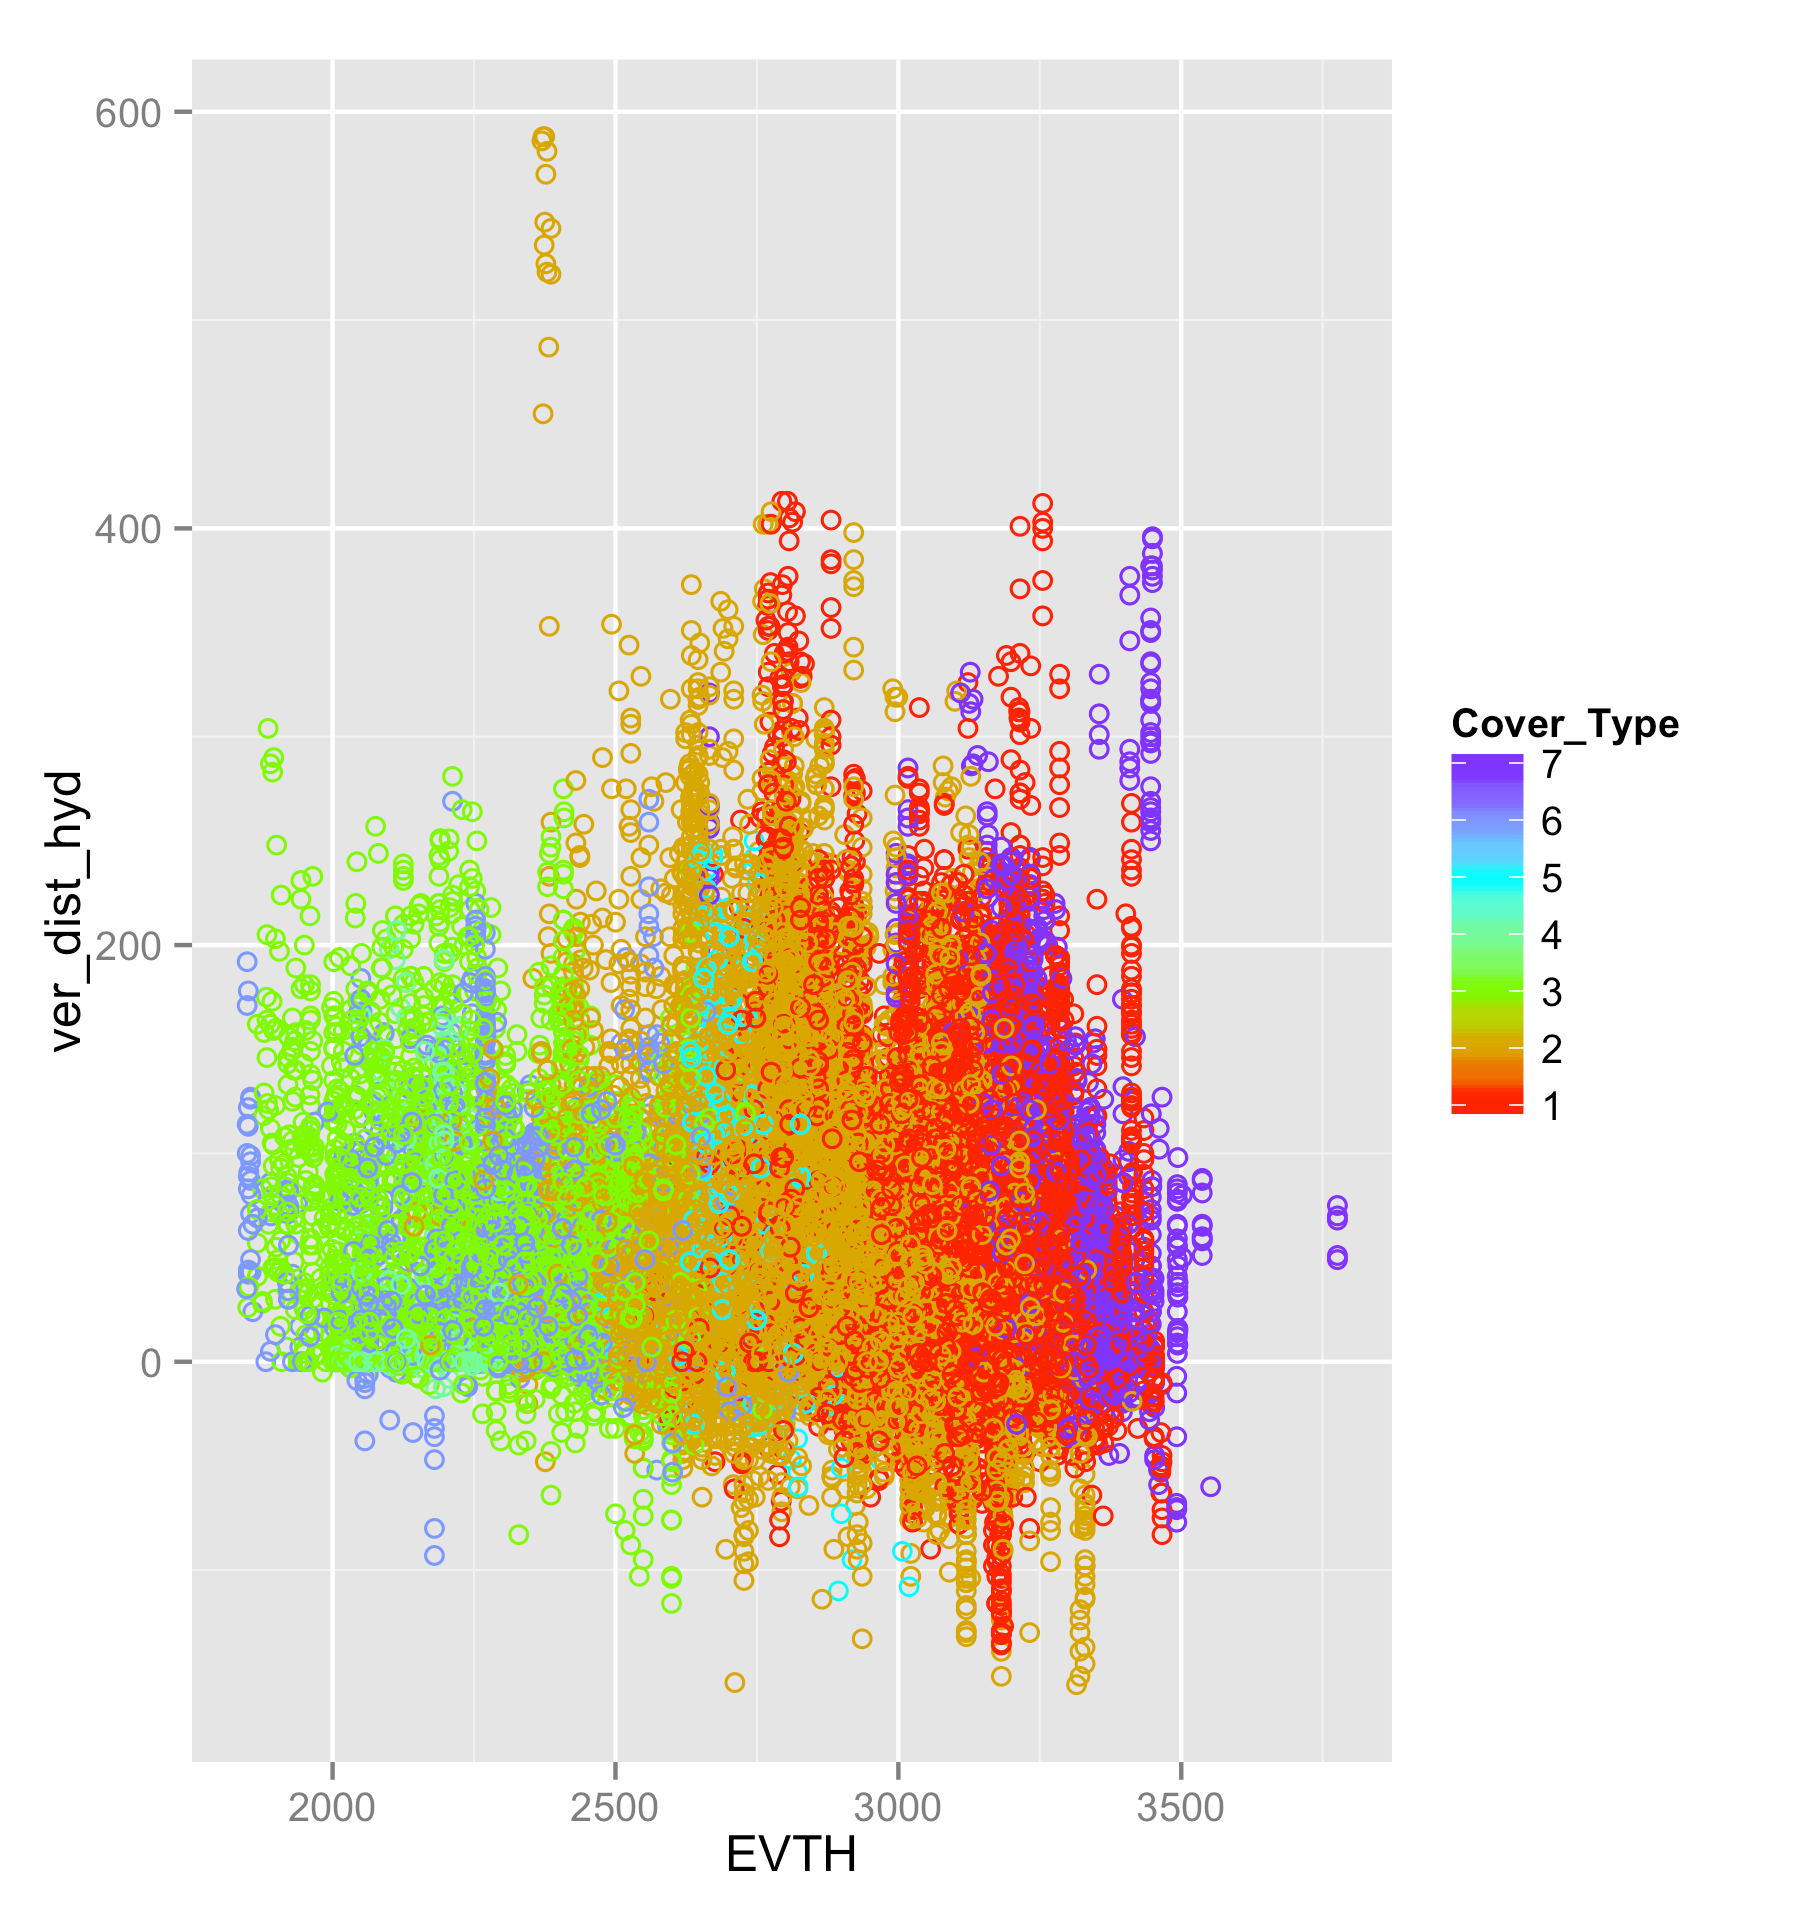
\includegraphics[width=0.8\textwidth]{EVTH_ver.png}
    \caption{ \textbf{IEVTH vs. \lstinline{vert_dist_hyd}}}
    \label{fig:errors}
\end{figure}

The created feature seems to separates the groups well. We observed a similar relationship between the horizontal distance and elevation and thus add the following variable.\\

Variable creation 2 (EDTH)\
\begin{lstlisting}
data$EDTH <- data$elevation - data$hor_dist_hyd*0.2
\end{lstlisting}
Using the same reasoning we observe and create the following variables.
Variable creation 3-6\
\begin{lstlisting}
data$Hydro_Road_1 <- abs(data$hor_dist_hyd + data$hor_dist_road)
\end{lstlisting}
\begin{lstlisting}
data$Fire_Road_1 <- abs(data$hor_dist_fire +data$hor_dist_road)
\end{lstlisting}
\begin{lstlisting}
data$hydro_road_2 <-  abs(data$hor_dist_hyd - data$hor_dist_road)
\end{lstlisting}
\begin{lstlisting}
data$Fire_Road_2 <- abs(data$hor_dist_fire - data$hor_dist_road)
\end{lstlisting}

\subsection{Variable creation}
Another variable which we suspect to add predictive power is the total distance to hyd.\\
\begin{lstlisting}
data$tot_dist_hyd <- sqrt((data$hor_dist_hyd)^2 + (data$ver_dist_hyd)^2)
\end{lstlisting}

\subsection{Variable transformation}
The aspect variable is circular and needs to be adjusted accordingly. We do that by shifting all values over 180 by 180.
Variable creation 7
\begin{lstlisting}
data$aspect_shifted <- ifelse(data$aspect > 180, data$aspect - 180 , data$aspect)
\end{lstlisting}
 % % % % % % % % % % % % % % % % % % % % % % % % % % % % % % % % % % % %





\newpage


 % % % % % % % % % % % % % % % % % % % % % % % % % % % % % % % % % % % %


\section{Methods}
\subsection{K-Nearest Neighbor}
With this method\footnote{Firstly proposed by Fix and Hodges (1951) \cite{knn}}, we try to classify each new observation in the test set taking into consideration the majority label from K nearest neighbors. In our case, we used the Euclidean distance as a measure of closeness between observations.


\subsection{Support Vector Machine}
This algorithm\footnote{SVM was firstly proposed by  Vapnik, V. and Chervonenkis, A. (1963) and soft SVM was proposed by  Cortes C. and Vapnik, V. (1995) \cite{vap}}  tries to predict the labels of the data set by separating the space into halfspaces - where in each halfspace we have different labels - with the largest margin (separation) possible. We can also introduce a cost parameter which tends to penalize the misclassification done within the bands. 

\subsection{Gradient Boosting}
This is an algorithm\footnote{Created by Friedman, J. H. (1999) \cite{Friedman00greedyfunction}} for predicting labels which combines different weak prediction functions to create one which is stronger, and in our case we used decision trees. So, it tries to find the best classifier by weighting different functions and considering a shrinkage parameter. Those weights are updated considering the misclassifications. 


\subsection{Random Forest}
This method \footnote{Firstly proposed by Breiman, L. (2001) \cite{random} } tries to create a strong classifier from the weighted sum of different decision trees. In each iteration it considers a random sample in the training set and fits a decision tree. Then, it considers small subsets of the features and divide the space considering thevariable that best separates the space. We do this procedure for many iterations. 


\subsection{Random Forest with deep learning}
This  method tries to combine the benefits from the Random Forest with the benefits from Deep learning. It takes into account that the data might have some hidden layers that transform the data. 



\newpage




 % % % % % % % % % % % % % % % % % % % % % % % % % % % % % % % % % % % %

\section{Experiments}
In a first set of experiments, we consider several well established classes of hypothesis functions. In particular, we consider Random Forests, Support Vector Machines, k-NN,  Gradient Tree Boosting and Neural Nets (Deep Learning). 
We first run these over a grid of hyperparameters without any feature engineering. This gives us a feeling for how well different methods are suited for the task at hand. In grid search, one evaluates a classifier over a grid, i.e. the cartesian product of several hyper parameter ranges. This process is computationally intensive, but since the data set is small, we can afford this luxury. The code for these experiments can be found in the files \lstinline{h2o_gridsearches.R}, \lstinline{svm_experiments.R} and \lstinline{knn_experiments.R}. The following figure shows the accuracy of the best model in each class. For the deep learning models, we try Tanh and Rectifier activation functions, over 15 and 20 epochs. We try 3 and 4 hidden layers with each 200 hidden units and a no vs a small l1 regularization. The best model has 3 hidden layers, no regularization and uses a Tanh activation. For the random forest, we try 40,80,100, 150, 200 trees where 100 work best. For the gbm we consider interaction depths of 3, 5, and 7, and 40, 60 and 120 boosting iterations, where a depth of 7 and 120 boosting iterations work best. 

\begin{figure}[H]
    \centering
    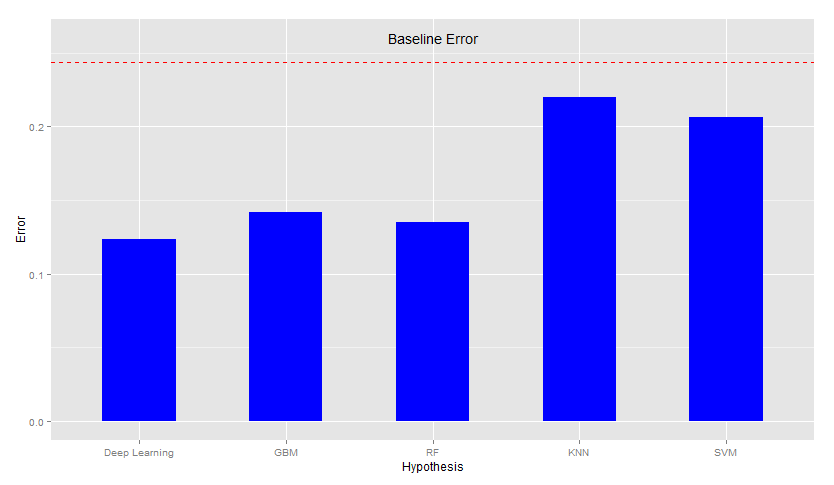
\includegraphics[width=0.8\textwidth]{erorrs.png}
    \caption{ \textbf{Initial errors}}
    \label{fig:errors}
\end{figure}

We clearly see that the performance of SVM and k-NN, at least in the tried configuration with this set of features is rather disappointing. Tree based methods  and neural nets however, show - with some parameter tuning - a significant improvement over the baseline. 
 


 % % % % % % % % % % % % % % % % % % % % % % % % % % % % % % % % % % % %
\newpage

\section{Feature Engineering and Model Tuning}
We settle on Deep Learning and Random Forests, since those performed best in the initial series of experiments. Based on our exploratory analysis, we add three new features to the data set: Horizontal Distance to Hydrology (water), Vertical Distance to Hydrology, and Total Distance to Hydrology. We feed these into the our previously best performing models, which leaves us with a slight gain in accuracy. 
Since Deep Learning seems to perform well for this data set, we try a heuristic: Why not train the Random Forest on features extracted with Deep Learning? The recent success on Deep Learning seems to be partly based on it's ability to abstract high-level concepts from the data. For this reason, Machine Learning researchers use it for feature, or representation learning. Feature learning can be done in a supervised or unsupervised manner. We use it in a supervised manner based on the heuristic: the neural net with the highest accuracy will provide the best features for our random forest. Operatively, what is done is just that the nodes of the last hidden layer in the neural net are extracted and used to transform the original feature space. The following figure shows the accuracy of all methods described: Random Forests, Deep Learning, and Random Forests with "Deep Features". 


We see that this results in a significant gain in accuracy. Apparently, Deep Learning is able to extract useful features from the data. However, in our last example we trained the random forest on 200 features. Too many features may potentially cause overfitting. This is why, in the next series of experiments, we add another layer to the neural net, where the size is significantly reduced, thus enforcing sparseness in the output. We try this with 50, 30 and 20 neurons. 


 % % % % % % % % % % % % % % % % % % % % % % % % % % % % % % % % % % % %


\section{Limitations}
Some of the main limitations in this project are, firstly, the computational power that we used although we had only a small dataset. This required us to use Amazon Web Service (AWS) in order to speed up our calculations. \\
Moreover, it was also hard to try to understand what was going on with this high-dimensional data. It would be easier if we have two or three dimensional data which we could visualize and better analyze what going on. \\
Furthermore, we have not tried to analyze the potential distribution under the data, in order to find causality measures in future which might give us insights of how forests work in nature. 
Finally, we have no clear idea if we might have jointly overfitted the cross - and visbile test set. 


 % % % % % % % % % % % % % % % % % % % % % % % % % % % % % % % % % % % %

\section{Conclusions}
Using a 50,000 observations training set as training and a 100,000 observations testing set, we try to classify 7 different classes using different machine learning methods such as K-NN, GBM or Random Forest.\\
We consider that the best classifier for this type of data is Random Forest with deep learning, which gives the smallest cross-validation error. 

\newpage
 % % % % % % % % % % % % % % % % % % % % % % % % % % % % % % % % % % % %
\bibliography{randombib}
	\bibliographystyle{plain}


\end{document}
 % % % % % % % % % % % % % % % % % % % % % % % % % % % % % % % % % % % %
 % % % % % % % % % % % % % % % % % % % % % % % % % % % % % % % % % % % %
 % % % % % % % % % % % % % % % % % % % % % % % % % % % % % % % % % % % %
